% Created by tikzDevice version 0.12.6 on 2026-05-14 19:27:22
% !TEX encoding = UTF-8 Unicode
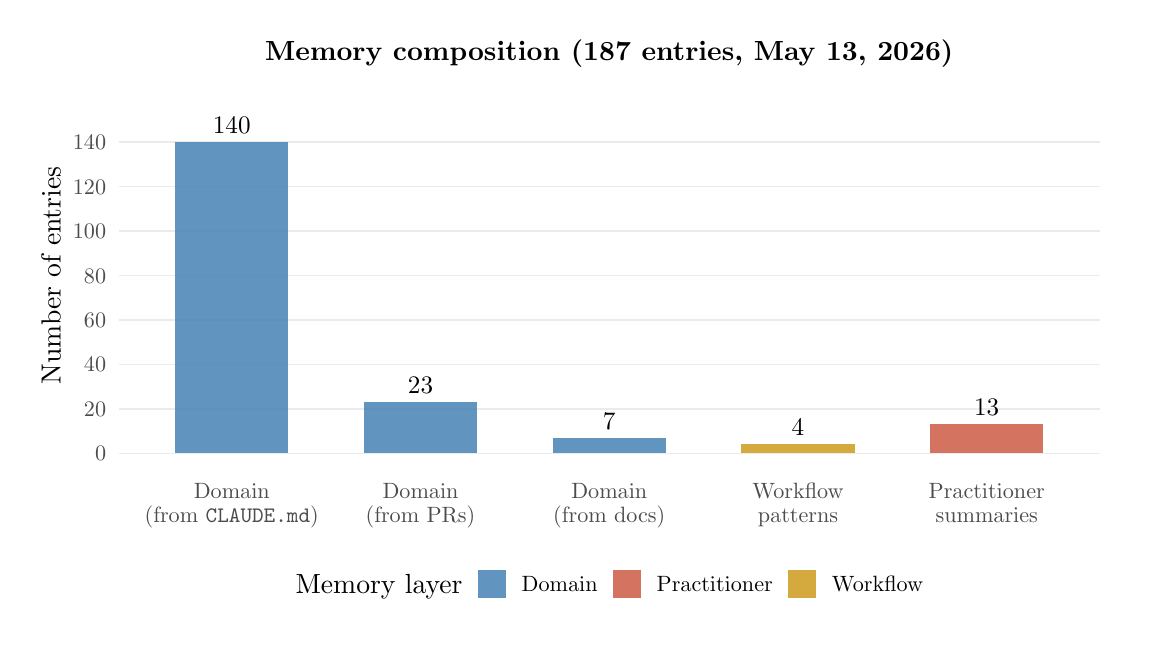
\begin{tikzpicture}[x=1pt,y=1pt]
\definecolor{fillColor}{RGB}{255,255,255}
\path[use as bounding box,fill=fillColor,fill opacity=0.00] (0,0) rectangle (397.48,216.81);
\begin{scope}
\path[clip] (  0.00,  0.00) rectangle (397.48,216.81);
\definecolor{fillColor}{RGB}{255,255,255}

\path[fill=fillColor] ( -0.00,  0.00) rectangle (397.48,216.81);
\end{scope}
\begin{scope}
\path[clip] ( 32.83, 56.59) rectangle (387.48,197.96);
\definecolor{drawColor}{gray}{0.92}

\path[draw=drawColor,line width= 0.5pt,line join=round] ( 32.83, 63.01) --
	(387.48, 63.01);

\path[draw=drawColor,line width= 0.5pt,line join=round] ( 32.83, 79.08) --
	(387.48, 79.08);

\path[draw=drawColor,line width= 0.5pt,line join=round] ( 32.83, 95.14) --
	(387.48, 95.14);

\path[draw=drawColor,line width= 0.5pt,line join=round] ( 32.83,111.21) --
	(387.48,111.21);

\path[draw=drawColor,line width= 0.5pt,line join=round] ( 32.83,127.28) --
	(387.48,127.28);

\path[draw=drawColor,line width= 0.5pt,line join=round] ( 32.83,143.34) --
	(387.48,143.34);

\path[draw=drawColor,line width= 0.5pt,line join=round] ( 32.83,159.41) --
	(387.48,159.41);

\path[draw=drawColor,line width= 0.5pt,line join=round] ( 32.83,175.47) --
	(387.48,175.47);
\definecolor{fillColor}{RGB}{70,130,180}

\path[fill=fillColor,fill opacity=0.85] ( 53.29, 63.01) rectangle ( 94.21,175.47);

\path[fill=fillColor,fill opacity=0.85] (121.49, 63.01) rectangle (162.41, 81.49);

\path[fill=fillColor,fill opacity=0.85] (189.70, 63.01) rectangle (230.62, 68.64);
\definecolor{fillColor}{RGB}{205,155,29}

\path[fill=fillColor,fill opacity=0.85] (257.90, 63.01) rectangle (298.82, 66.23);
\definecolor{fillColor}{RGB}{205,91,69}

\path[fill=fillColor,fill opacity=0.85] (326.10, 63.01) rectangle (367.02, 73.46);
\definecolor{drawColor}{RGB}{0,0,0}

\node[text=drawColor,anchor=base,inner sep=0pt, outer sep=0pt, scale=  0.91] at ( 73.75,178.61) {140};

\node[text=drawColor,anchor=base,inner sep=0pt, outer sep=0pt, scale=  0.91] at (141.95, 84.62) {23};

\node[text=drawColor,anchor=base,inner sep=0pt, outer sep=0pt, scale=  0.91] at (210.16, 71.77) {7};

\node[text=drawColor,anchor=base,inner sep=0pt, outer sep=0pt, scale=  0.91] at (278.36, 69.36) {4};

\node[text=drawColor,anchor=base,inner sep=0pt, outer sep=0pt, scale=  0.91] at (346.56, 76.59) {13};
\end{scope}
\begin{scope}
\path[clip] (  0.00,  0.00) rectangle (397.48,216.81);
\definecolor{drawColor}{gray}{0.30}

\node[text=drawColor,anchor=base east,inner sep=0pt, outer sep=0pt, scale=  0.80] at ( 28.33, 60.26) {0};

\node[text=drawColor,anchor=base east,inner sep=0pt, outer sep=0pt, scale=  0.80] at ( 28.33, 76.32) {20};

\node[text=drawColor,anchor=base east,inner sep=0pt, outer sep=0pt, scale=  0.80] at ( 28.33, 92.39) {40};

\node[text=drawColor,anchor=base east,inner sep=0pt, outer sep=0pt, scale=  0.80] at ( 28.33,108.45) {60};

\node[text=drawColor,anchor=base east,inner sep=0pt, outer sep=0pt, scale=  0.80] at ( 28.33,124.52) {80};

\node[text=drawColor,anchor=base east,inner sep=0pt, outer sep=0pt, scale=  0.80] at ( 28.33,140.59) {100};

\node[text=drawColor,anchor=base east,inner sep=0pt, outer sep=0pt, scale=  0.80] at ( 28.33,156.65) {120};

\node[text=drawColor,anchor=base east,inner sep=0pt, outer sep=0pt, scale=  0.80] at ( 28.33,172.72) {140};
\end{scope}
\begin{scope}
\path[clip] (  0.00,  0.00) rectangle (397.48,216.81);
\definecolor{drawColor}{gray}{0.30}

\node[text=drawColor,anchor=base,inner sep=0pt, outer sep=0pt, scale=  0.80] at ( 73.75, 46.58) {Domain};

\node[text=drawColor,anchor=base,inner sep=0pt, outer sep=0pt, scale=  0.80] at ( 73.75, 37.94) {(from \texttt{CLAUDE.md})};

\node[text=drawColor,anchor=base,inner sep=0pt, outer sep=0pt, scale=  0.80] at (141.95, 46.58) {Domain};

\node[text=drawColor,anchor=base,inner sep=0pt, outer sep=0pt, scale=  0.80] at (141.95, 37.94) {(from PRs)};

\node[text=drawColor,anchor=base,inner sep=0pt, outer sep=0pt, scale=  0.80] at (210.16, 46.58) {Domain};

\node[text=drawColor,anchor=base,inner sep=0pt, outer sep=0pt, scale=  0.80] at (210.16, 37.94) {(from docs)};

\node[text=drawColor,anchor=base,inner sep=0pt, outer sep=0pt, scale=  0.80] at (278.36, 46.58) {Workflow};

\node[text=drawColor,anchor=base,inner sep=0pt, outer sep=0pt, scale=  0.80] at (278.36, 37.94) {patterns};

\node[text=drawColor,anchor=base,inner sep=0pt, outer sep=0pt, scale=  0.80] at (346.56, 46.58) {Practitioner};

\node[text=drawColor,anchor=base,inner sep=0pt, outer sep=0pt, scale=  0.80] at (346.56, 37.94) {summaries};
\end{scope}
\begin{scope}
\path[clip] (  0.00,  0.00) rectangle (397.48,216.81);
\definecolor{drawColor}{RGB}{0,0,0}

\node[text=drawColor,rotate= 90.00,anchor=base,inner sep=0pt, outer sep=0pt, scale=  1.00] at ( 11.89,127.28) {Number of entries};
\end{scope}
\begin{scope}
\path[clip] (  0.00,  0.00) rectangle (397.48,216.81);
\definecolor{drawColor}{RGB}{0,0,0}

\node[text=drawColor,anchor=base west,inner sep=0pt, outer sep=0pt, scale=  1.00] at ( 96.79, 12.25) {Memory layer};
\end{scope}
\begin{scope}
\path[clip] (  0.00,  0.00) rectangle (397.48,216.81);
\definecolor{fillColor}{RGB}{70,130,180}

\path[fill=fillColor,fill opacity=0.85] (162.76, 10.65) rectangle (172.85, 20.73);
\end{scope}
\begin{scope}
\path[clip] (  0.00,  0.00) rectangle (397.48,216.81);
\definecolor{fillColor}{RGB}{205,91,69}

\path[fill=fillColor,fill opacity=0.85] (211.58, 10.65) rectangle (221.67, 20.73);
\end{scope}
\begin{scope}
\path[clip] (  0.00,  0.00) rectangle (397.48,216.81);
\definecolor{fillColor}{RGB}{205,155,29}

\path[fill=fillColor,fill opacity=0.85] (274.88, 10.65) rectangle (284.97, 20.73);
\end{scope}
\begin{scope}
\path[clip] (  0.00,  0.00) rectangle (397.48,216.81);
\definecolor{drawColor}{RGB}{0,0,0}

\node[text=drawColor,anchor=base west,inner sep=0pt, outer sep=0pt, scale=  0.80] at (178.49, 12.94) {Domain};
\end{scope}
\begin{scope}
\path[clip] (  0.00,  0.00) rectangle (397.48,216.81);
\definecolor{drawColor}{RGB}{0,0,0}

\node[text=drawColor,anchor=base west,inner sep=0pt, outer sep=0pt, scale=  0.80] at (227.31, 12.94) {Practitioner};
\end{scope}
\begin{scope}
\path[clip] (  0.00,  0.00) rectangle (397.48,216.81);
\definecolor{drawColor}{RGB}{0,0,0}

\node[text=drawColor,anchor=base west,inner sep=0pt, outer sep=0pt, scale=  0.80] at (290.62, 12.94) {Workflow};
\end{scope}
\begin{scope}
\path[clip] (  0.00,  0.00) rectangle (397.48,216.81);
\definecolor{drawColor}{RGB}{0,0,0}

\node[text=drawColor,anchor=base,inner sep=0pt, outer sep=0pt, scale=  1.00] at (210.16,204.91) {\bfseries Memory composition (187 entries, May 13, 2026)};
\end{scope}
\end{tikzpicture}
